% Niniejszy plik stanowi przykład formatowania pracy magisterskiej na
% Wydziale MIM UW.  Szkielet użytych poleceń można wykorzystywać do
% woli, np. formatujac wlasna prace.
%
% Zawartosc merytoryczna stanowi oryginalnosiagniecie
% naukowosciowe Marcina Wolinskiego.  Wszelkie prawa zastrzeżone.
%
% Copyright (c) 2001 by Marcin Woliński <M.Wolinski@gust.org.pl>
% Poprawki spowodowane zmianami przepisów - Marcin Szczuka, 1.10.2004
% Poprawki spowodowane zmianami przepisow i ujednolicenie 
% - Seweryn Karłowicz, 05.05.2006
% Dodanie wielu autorów i tłumaczenia na angielski - Kuba Pochrybniak, 29.11.2016

% !TeX spellcheck = en_GB
\documentclass[en]{pracamgr}
\usepackage{amsfonts, color, soul, amsmath}
\usepackage{float}
\usepackage{graphicx}
\graphicspath{ {./graphics/} }
% Dane magistrantów:
\autor{Marek Wieczorek}{426777}
%\autori{Autor Pierwszy}{342013}
%\autorii{Drugi Autor-Z-Rzędu}{231023}
%\autoriii{Trzeci z Autorów}{777321}
%\autoriv{Autor nr Cztery}{432145}
%\autorv{Autor nr Pięć}{342011}

\title{Title in English}
\titlepl{Tytuł po polsku}

%\tytulang{An implementation of a difference blabalizer based on the theory of $\sigma$ -- $\rho$ phetors}

%kierunek: 
% - matematyka, informacyka, ...
% - Mathematics, Computer Science, ...
\kierunek{Computational Engineering}

% informatyka - nie okreslamy zakresu (opcja zakomentowana)
% matematyka - zakres moze pozostac nieokreslony,
% \zakres{Tu wpisac, jesli trzeba, jedna z opcji podanych wyzej}

% Praca wykonana pod kierunkiem:
% (podać tytuł/stopień imię i nazwisko opiekuna
% Instytut
% ew. Wydział ew. Uczelnia (jeżeli nie MIM UW))
\opiekun{dr Marek Michalewicz}

% miesiąc i~rok:
\date{May 2021}

%Podać dziedzinę wg klasyfikacji Socrates-Erasmus:
\dziedzina{ 
%11.0 Matematyka, Informatyka:\\ 
%11.1 Matematyka\\ 
%11.2 Statystyka\\ 
11.3 Informatyka\\ 
%11.4 Sztuczna inteligencja\\ 
%11.5 Nauki aktuarialne\\
%11.9 Inne nauki matematyczne i informatyczne
}

%Klasyfikacja tematyczna wedlug AMS (matematyka) lub ACM (informatyka)
\klasyfikacja{D. Software\\
  D.127. Blabalgorithms\\
  D.127.6. Numerical blabalysis}

% Słowa kluczowe:
\keywords{quantum annealing, D-Wave}

% Tu jest dobre miejsce na Twoje własne makra i~środowiska:
%\newtheorem{defi}{Definicja}[section]

% koniec definicji

\begin{document}
\maketitle

%tu idzie streszczenie na strone poczatkowa
\begin{abstract}
Here an abstract will show up in some months to follow.
\end{abstract}

\tableofcontents
%\listoffigures
%\listoftables

\chapter{Introduction}
There is probably no single point in space-time where the concept of \textit{quantum computing} emerged for the very first time. In the 70' Paul Benioff was investigating the topic and in year 1980 published a foundational article \textit{The computer as a physical system: A microscopic quantum mechanical Hamiltonian model of computers as represented by Turing machines}\cite{benioff_computer_1980}. But it took celebrity-physicist and Nobel Prize winner Richard Feynman to mark the beginning of the discipline (for sure anegdoticaly). He discussed the topic in 1981 talk \textit{Simulating physics with computers} during a small conference on the topic of \textit{Physics of Computation} held at MIT. Present were also Paul Benioff and other scientists whose work contributed to the birth of the discipline: Rolf Landauer and Tom Toffoli \cite{mit_endicott_house_physics_2018}. In his foundational talk, Feynman indicated that for an efficient simulation of quantum phenomena, a different kind of computer was needed. The reasoning behind the idea is that quantum systems description grows exponentially with the number of particles involved. A system large enough will quickly overwhelm any classical computer. The conclusion of the talk:
\begin{quote}
Nature isn't classical, dammit, and if you want to make a simulation of Nature, you'd better make it quantum mechanical, and by golly it's a wonderful problem because it doesn't look so easy \cite{feynman_simulating_1982}.
\end{quote}
became famous and is often treated as a spark that ignited the discipline \cite{john_preskill_feynman_2017}\cite{trabesinger_quantum_2012}\cite{the_quantum_insider_global_2021}:
\begin{quote}
With those words, in 1981, Richard Feynman, an American physicist, introduced the idea that, by harnessing quantum mechanics, it might be possible to build a new kind of computer, capable of tackling problems that would cause a run-of-the-mill machine to choke \cite{the_economist_google_2019}.
\end{quote}
Following years have seen a gradual development of the ideas, with formalisation of the notion of a quantum computer by David Deutsch\cite{david_deutsch_quantum_1985} and other important results, all theoretical. Major breakthrough came in 1994 when Peter Shor demonstrated a quantum algorithm for efficient factorisation of big numbers. As modern cryptography (RSA public key encryption) relies on prohibitive cost of factorizing large enough numbers, the implications of the proposed algorithm were clear and caused quantum computing to draw major attention.
Some like Rolf Landauer shared their scepticism whether an effective quantum computer could be ever built. They pointed out that discussed approaches required perfect devices, neglecting effects such as \textit{quantum decoherence}. Peter Shore was again the one to make a major contribution by proposing quantum error-correction. He proved, that a quantum code could be executed effectively even if errors occur, given that they are sufficiently rare. This of course comes at a cost --- a big computational overhead.

At this stage, the theory was clearly ahead of the hardware, but the attempts to build quantum computer have been made. \textbf{What was the first practical attempt?}
Digital vs. analog? How to introduce D-Wave into the topic? Is it the first quantum computer?

\section{Gate model}
Some text about the gate model computers

\subsection{Error correction}
Some for subsection of error correction
\section{Quantum Annealing}
Quantum annealing has some interesting properties. It is analog in nature and because the computation happens in a ground state it is unaffected by decoherence \cite{mcgeoch2014adiabatic}.
Quantum annealing is a computational process, an optimization metaheuristic proposed theoretically in 1988 in \cite{apolloni1988numerical}, as an analogy to simulated annealing, formulated five years earlier \cite{kirkpatrick1983optimization}. It was first simulated classically, to finally become realised in an analog hardware by D-Wave Inc. First working quantum annealer was presented in 2007 and contained 16 qubits \cite{d-wave_inc_d-wave_2007}. To fully understand the term and to develop a bottom-up intuition of the process it is best to track the gradual development of the concept.
\subsection{Thermal Annealing} \label{sub:thermal_annealing}
Traditionally annealing refers to thermal annealing, a metallurgical process known to humanity for centuries. Annealing reduces hardness and increases ductility of a (most often) metal peace, making it more workable. The peace is heated until glowing (for steel) and kept in high temperature. The temperature increases the rate at which atoms diffuse in the metal, eradicating dislocations of the crystalline structure, hence moving towards equilibrium state - lower internal stresses. Lower number of dislocations results in higher ductility. The process of stress-relief is spontaneous, so it also progresses at room temperature, although at a very slow pace. It is the heat that increases the energy of thermal fluctuations, making transitions more probable. This concept is the basis on which, by analogy, optimisational algorithms were build. Annealing may also be applied to glass, with similar purposes and process. As glass has no crystalline structure, the mechanics differ \cite{wikipedia_contributors_annealing_2021}.

A process with opposite effects is quenching, where hot material is cooled rapidly. This results in sub-optimal configuration of the material. Remaining stresses make the material harder but more brittle \cite{wikipedia_contributors_quenching_2021}.
\subsection{Simulated Annealing}
As an optimizational algorithm, simulated annealing emerged in the early '80 in a paper by Kirkpatrick, Gelatt, and Vecchi \cite{kirkpatrick1983optimization}. As of 2021, it was cited almost 50\,000 times, indicating how influential the idea is. The work of Kirkpatrick et al. is based on much older concept, the Metropolis algorithm by Metropolis et al. \cite{metropolis1953equation}. The authors devised a computational method for studying aggregate properties of the large number of particles, a subject of the statistical mechanics. As the number of particles is typically big (an order of $10^23/cm^3$) only the most probable behaviour of the system is observed in the experiments. To calculate parameters of this observable state, a Gibbs ensemble is used. It is an average of a parameter taken over all possible configurations, each defined by particle positions and weighted by a corresponding Boltzmann probability factor:
\[p\propto e^{-E/kT}\]
where $k$ is the Boltzmann constant, $T$ is temperature, $E$ the potential energy of the configuration, defined as:
\[E=\frac{1}{2}\sum_{i=1}^{N}\sum_{j=1}^{N}V(d_{ij})\]
where $V$ is the potential between particles, $d$ is the distance between them.

The averaging involves integration over a high-dimensional configuration space. As the number of particles is high, so is the dimensionality of the integral. Metropolis et al. proposed a computational method for tackling the problem of integration, based on Monte Carlo method. They studied a group of interacting particles (56 or 224) packed in a two-dimensional, closed space, at a given temperature. Standard Monte Carlo method involves random, uniform sampling of points and assigning them a weight which represents the probability of finding a particular configuration. Any randomly selected state will most probably be far from "optimum", hence with high energy and finally with low weight (probability) assigned. Standard Monte-Carlo method which involves sampling from a uniform distribution would require a huge number of configurations to be calculated, most of which with a very low contribution. Instead the authors choose configurations with probability $e^{-E/kT}$ and weight them evenly.

The algorithm starts from a random particle configuration of the particles, next following steps are executed in a loop :
\begin{enumerate}
	\item Move a chosen particle to new positions:
		\[X\rightarrow X+\alpha\gamma_1\]
		\[Y\rightarrow Y+\alpha\gamma_2\]
	where $X$, $Y$ are the coordinates of the particle, $\alpha$ is the maximum allowed step, $\gamma_1$ and $\gamma_2$ are random numbers between $-1$ and $1$.
	\item Calculate the change in energy $\Delta E$. If $\Delta E<0$ the move is always allowed, so we always accept "better" solution. If $\Delta E>0$ the move is allowed with probability $e^{-E/kT}$. To realise the probability, $\gamma_3$ between $0$ and $1$ is randomly selected. If $\gamma_3<e^{-E/kT}$ the move is accepted, else rejected.
	\item Whether the configuration has changed or not, each step is taken into account for counting the ensembles.
\end{enumerate}
The described algorithm allows for studying the properties of a set of particles at a given temperature. There is a connection with optimisation as we have discussed states of lower energy, the optimal ones. Still there is a little chance of finding them randomly. So how to transform a computational method of statistical mechanics into a optimisation algorithm? Kirkpatrick et al. realised that by lowering the temperature of the algorithm, one would simulate cooling process. At the end of the process, the Boltzmann distribution collapses into the lowest energy states.
%% TUTAJ wykres rozkładu boltzmanna p(T) dla E=10 i E=1000
Unfortunately, low temperature is not a sufficient condition for finding  the optimal state. Please refer to section \ref{sec:thermal_annealing} for detailed description of thermal processes. Rapid cooling is a process called quenching where sub-optimal state, a local minimum is produced. Process of slow cooling aiming at releasing residual stresses in the material is annealing. When done slow enough, it results in an optimal material configuration. Hence the name of the algorithm \emph{simulated annealing}.

The process of annealing clearly is a method of optimizing the material configuration. To universally apply it to optimisation problems it is important to clarify the idea of temperature, energy and the Boltzmann constant. All these values have a clear meaning in thermodynamics but in an algorithmic sense they relate to progress parameter, cost function and a coefficient.


\subsection{Quantum Annealing}

\chapter{How to Use Quantum Annealing}
\section{Problem Description}
Quantum annealing allows for solving a wide range of optimisation problems. A common description of the problems is needed to allows for easy comparison, tooling compatibility but also to determine what is solvable with the available equipment. This section discusses two most common descriptions which are interchangeable.
\subsection{Lenz-Ising Model}
The model is most often called \textit{Ising model} after Ernst Ising. In his brief paper from 1925 he clearly states that he developed a concept first proposed by his research director --- Wilhelm Lenz in 1920\cite{ising_beitrag_1925}. Hence I follow naming used by Brush and Niss\cite{brush_history_1967}\cite{niss_history_2005}. Model proposed by Lenz assumed a magnetic material to be constituted of elementary micromagnets (as proposed in 1907 by P.~Weiss) but with an additional constraint that each micromagnet is only able to take two positions "up" and "down". Ising developed the model by considering nearest-neighbour interactions in a linear chain of micromagnets. Exact solution obtained by Ising showed that one-dimensional model was not capable of explaining the ferromagnetism. Erroneously, Ising concluded that his result was valid in three dimensions:
\begin{quote}
Es ist gezeigt, das für lineare Ketten und gewisse Modifikationen kein Ferromagnetismus unter den obigen Voraussetzungen entsteht. Es besteht die Vermutung, daß auch beim dreidimensionalen analogen Modell ein ferromagnetisches Verhalten nicht erzielt werden. \textit{(It is shown that for linear chains and certain modifications no ferromagnetic effect was achieved under the above conditions. It is assumed that also in case of a three-dimensional model, ferromagnetic behaviour will not be achieved)}\cite{ising_beitrag_1925}
\end{quote}
The ideas proposed by Lenz and Ising survived despite the lack of apparent success. In 1936 Rudolf Peierls showed that for a two-dimensional case the model indeed is capable of explaining the ferromagnetism. Progress in other areas of study such as binary alloys and transition points resulted in formulation of descriptions mathematically equivalent to Lenz-Ising model. To describe any of these phenomena in a system, one has to consider joint action of units the system is composed of, hence the term \textit{cooperative phenomena}. Finally in 1944 Rals Onsager published a paper titled \textit{A Two-Dimensional Model with an Order-Disorder Transition}. He provided a mathematical proof that two-dimensional Lenz-Ising model is capable of explaining ferromagnetism. The history of Lenz-Ising model is very interesting and often surprising. Please refer to Brush \cite{brush_history_1967} and Niss\cite{niss_history_2005} for a detailed description.

The model, however basic and idealised, proved to offer a great trade-off between realism and mathematical usability. This resulted in its great success both in terms of citations (thousands for papers of Ising and Onsager) but also a growing number of areas it is used in. One of proofs of this success is the important role the model currently plays in the area of combinatorial optimisation.

\hl{the model below is a hamiltonian. How did the original concept end up being hamiltonian?}

\hl{modern version of the model description}

\[H(\sigma) = -\sum_{\langle i~j\rangle} J_{ij} \sigma_i \sigma_j - \mu \sum_j h_j \sigma_j,\]

\subsection{QUBO}
Quadratic Unconstrained Binary Optimisation (QUBO) is an NP-hard combinatorial optimisation problem. It serves as a general mathematical description for many widely studied and relevant problems such as: \hl{Travelling Salesman Problem, Max-cut problem, Map coloring}.  In general form it is defined as:
\[f_Q(x) = \sum_{i=1}^n \sum_{j=1}^i q_{ij} x_i x_j\]
with $x_i\in\lbrace 0,1\rbrace$ for $i\in[n]$ and coefficients $q_{ij}\in\mathbb{R}$ for $1\leq j\leq i\leq n$.

An equivalent matrix notation of QUBO is:
\[ min\ y=x^\top Qx\]
where $Q\in\mathbb{R}^{n\times n}$ is the symmetric $n\times n$ matrix containing the coefficients $q_{ij}$.

In general, QUBO is a minimisation problem, but if $f(x)$ is a function to be maximised, it is sufficient to minimise $-f(x)$. By being a mathematical description of wide use, it is similar to Lenz-Ising model. Interestingly both descriptions are interchangeable.

\subsubsection{Natural QUBO formulations}
\label{subsub:natural_qubo}
Some of combinatorial problems fit QUBO "naturally" without any tricks. This is true for problems that do not have any constraints. One example of such problem is Number Partitioning. In common definition, its goal is to divide a set of numbers so the respective sums of the two resulting subsets are close to each other as possible. Given a set of numbers $S=\lbrace s_1,s_2,...,s_m\rbrace$, let $x_i=1$ if $s_i$ is assigned to set 1, $x_i=0$ otherwise. The sum for subset 1 is given as $sum_1=\sum_{i=1}^ms_ix_i$ and the sum for subset 2 is $sum_2=\sum_{i=1}^ms_i - \sum_{i=1}^ms_ix_i$. The difference:
\[diff=sum_1-sum_2=\sum_{i=1}^ms_i - 2\sum_{i=1}^ms_ix_i= c - 2\sum_{i=1}^ms_ix_i\]
Let us consider the square of the difference, hence minimum will be the optimum (0):
\[diff^2=\left(c - 2\sum_{i=1}^ms_ix_i\right)^2=c^2+4\sum_{i=1}^ms_ix_i\left(\sum_{i=1}^ms_ix_i-c\right)\]
Now we can drop constant values $c^2$ and $4$ and convert the sums into vectors and matrix:
\[min\ y =\sum_{i=1}^ms_ix_i\left(\sum_{i=1}^ms_ix_i-c\right)=
\sum_{i=1}^m s_i x_i(s_i x_i-c) + 2\sum_{i=1}^m \sum_{\substack{j=1 \\ j\ne i}}^m s_i x_i s_j x_j=
x^\top Qx\],
where $q_{ii}=s_i(s_i-c)$ and $q_{ij}=q_{ji}=s_is_j$. Elements of the $Q$ matrix diagonal correspond to $x_i^2$ terms. It is important to note that because for boolean variables $x^2=x$:
\[s_i x_i(s_i x_i-c) = s_i^2 x_i^2 - c s_i x_i = x_i^2 s_i(s_i - c)\]
Other examples of problems that naturally map to QUBO are Max-Cut Problem \hl{what else?}
\subsubsection{QUBO by reformulation}
Of course the majority of interesting problems do not map so easily to QUBO. Often, additional constraints are required which do not match the "unconstrained" description. The main idea of mapping such problems is not restricting the solution but increasing the cost of infeasible solutions by using penalties. Corresponding terms are added to the basic function. If the penalty terms reach zero, whole function becomes the original, unconstrained function. Great feature of QUBO is that it is additive in nature so ideally, the final solution will be in the intersection of minimums for all constituting terms of QUBO. Sometimes such solution does not exist and some trade-offs have to be made. An increased cost is acceptable but non-physical result is clearly not. This gradation of penalty terms is done by multiplying them with weights. More important constraint will result in a penalty term with a high weight. \autoref{tab:qubo1} presents common constraints and their corresponding penalties.

\begin{table}[h]
\begin{center}
\begin{tabular}{ l l }
 Classical constraint & Equivalent penalty\\ 
  \hline
 $x_1 + x_2 \le 1$ & $P(x_1x_2)$ \\  
 $x_1 + x_2 \ge 1$ & $P(1- x_1 - x_2 + x_1x_2)$ \\
 $x_1 + x_2 = 1$ & $P(1- x_1 - x_2 + 2x_1x_2)$ \\
 $x_1 \le x_2$ & $P(x_1 - x_1x_2)$ \\
 $x_1 + x_2 + x_3 \le 1$ & $P(x_1x_2 + x_2x_3 + x_3x_1)$ \\
 $x_1 = x_2$ & $P(x_1 + x_2 - 2x_1x_2)$ \\
\end{tabular}
\end{center}
\caption{Common constraints and their corresponding penalties.}
\label{tab:qubo1}
\end{table}

where $x_i\in\lbrace 0,1\rbrace$ and $P$ is penalty weight. Also logical constraints are possible. \autoref{tab:qubo2} presents them. When the equality is met, the penalty term is $0$. $x_3$ can be substituted with a constant value if needed.


\begin{table}[h]
\begin{center}
\begin{tabular}{ l l }
 Logical constraint & Equivalent penalty\\
  \hline 
 $NOT(x_1)=x_2$ & $P(2x_1x_2-x_1-x_2+1)$ \\  
 $AND(x_1, x_2)=x_3$ & $P(x_1x_2 - 2(x_1 + x_2)x_3 + 3x_3))$ \\
 $OR(x_1, x_2)=x_3$ & $P(x_2x_1 + (x_1+x_2)(1-2x_3)+x_3$) \\
\end{tabular}
\end{center}
\caption{Logical constraints and their corresponding penalties\cite{tanahashi_application_2019}\cite{zaman_pyqubo_2021}.}
\label{tab:qubo2}
\end{table}


For constructing more elaborate penalties, logical gates are also of use. Table \autoref{tab:qubo3} presents such gates and their corresponding penalties. Please note that $AND$ gate appeared in table \autoref{tab:qubo1}.
\begin{table}[h]
\begin{center}
\begin{tabular}{ l l }
 Logical gate & Equivalent penalty\\
 \hline
 $NOT(x_1)$ & $P(1-x_1)$ \\  
 $AND(x_1, x_2)$ & $P(x_1x_2)$ \\
 $OR(x_1, x_2)$ & $P(x_1+x_2-x_1x_2)$\\
\end{tabular}
\end{center}
\caption{Logical gates and their corresponding penalties \cite{tanahashi_application_2019}\cite{zaman_pyqubo_2021}.}
\label{tab:qubo3}
\end{table}

Now let us consider a practical example of Maximal Independent Set (equivalent to Set Packing). The task is best described as graph coloring problem: mark as many graph vertices so that no two colored vertices are connected by an edge. Let us define $x_i=1$ if vertex $i$ is colored, $x_i=0$ otherwise. The objective is:
\[max\ \sum_{i=1}^mx_i\]
with additional constraints that no two vertices sharing an edge are allowed, so penalty has to be applied if $AND(x_i, x_j)$. We can use \autoref{tab:qubo3} or \autoref{tab:qubo1} and formulate a set of constraints:
\[P\sum_{ij\in E}^m x_i x_j \]
finally, one has to remember that minimisation task should be considered, so finally:
\[min\ -\sum_{i=1}^mx_i + P\sum_{ij\in E}^m x_i x_j\]

\begin{figure}[h]
	\label{fig:graph_1}
	\caption{Simple graph with three edges.}
    \centering
    \def\svgwidth{0.25\textwidth}
    \input{graphics/graph_1.pdf_tex}
\end{figure}

For a particular graph presented in \autoref{fig:graph_1} the task becomes:
\[min\ \left[-\sum_{i=1}^4x_i + P\sum_{i=1}^3 x_i x_{i+1}\right]\]
\autoref{tab:qubo_results} contains QUBO values for all possible solutions and 3 values of penalty factor $P\in{1,2,3}$. Valid solutions (rows 1-5, 10 and 11) are unaffected by the value of $P$. This is easily explained by "switching-off" of the penalties for valid solutions. Row 12 is an interesting case: for $P=1$ is seems to be among the best solutions but that is not the case for any other value of $P$. Clearly, $P$ that is to low might not exclude invalid solutions. So should it then be much higher? Rightmost column contains solutions for $P=10$. Clearly the problem discussed earlier is solved, unfortunately other issue arises: the gap between best and second best solutions gets much smaller compared to overall range of possible values ($ \frac{1}{28}=3,6\% $). For $P=2$ the gap is $25\%$. \hl{when is it a problem? DWave 4bit precision? Is it for couplings or readout as well?}

\begin{table}
\begin{center}
\begin{tabular}{l | c c c c c c c }
row&$x1$&$x2$&$x3$&$x4$&$P=1$&$P=2$&$P=10$\\
 \hline
1&0&0&0&0&0&0&0\\ 
2&0&0&0&1&-1&-1&-1\\ 
3&0&0&1&0&-1&-1&-1\\
4&0&1&0&0&-1&-1&-1\\
5&1&0&0&0&-1&-1&-1\\ 
6&0&0&1&1&-1&0&8\\ 
7&0&1&0&1&-2&-2&-2\\ 
8&0&1&1&0&-1&0&8\\ 
9&0&1&1&1&-1&1&17\\ 
10&1&0&0&1&-2&-2&-2\\ 
11&1&0&1&0&-2&-2&-2\\ 
12&1&0&1&1&-2&-1&7\\ 
13&1&1&0&0&-1&0&8\\ 
14&1&1&0&1&-2&-1&7\\ 
15&1&1&1&0&-1&1&17\\ 
16&1&1&1&1&-1&2&26\\
\end{tabular}
\end{center}
\caption{All solution of Maximal Independent Set QUBO}
\label{tab:qubo_results}
\end{table}

\subsubsection{QUBO - graph equivalence}
\label{subsub:graph_equivalence}
Let us consider one more example: 3 binary variables $a$,$b$, $c$. Exactly one of them should be equal $1$. We can think of a constraint:
\[a+b+c=1\]
As we seek a minimization task, it is best to reformulate the constraint:
\[min(a+b+c-1)^2\]
Without this step, $a=0$, $b=0$, $c=0$ would make up the minimum, despite the fact that the original constraint is not satisfied. After expansion:
\[min(a^2+b^2+c^2+2ab+2ac+2bc-2a-2b-2c+1)\]
Note that for binary variables $x=x^2$, also a constant value increases or decreases all solution values by same amount, hence it can be omitted. Finally:
\[min(2ab+2ac+2bc-a-b-c)\]
Now let us change the notation:
\[min(-\sum_{i=1}^3x_i + 2\sum_{i=1}^3\sum_{\substack{j=1 \\ j\neq i}}^3 x_i x_j)\]
After this step it becomes clear that this is an example of QUBO. In previous example it was shown how to describe a graph problem with a QUBO, but the reverse is also possible. In fact, each QUBO describes a graph. This key property that is used by D-Wave quantum annealers - a graph is constructed in the hardware and its annealing takes place. A graph of current example is shown in \autoref{fig:dwave_triangle_graph}. $q_i$ coefficients describe node biases, $q_{ij}$ describe edge weights. Considering $i, j \in \{1,\ldots N\}$, it becomes clear that a universal hardware that allows to construct any QUBO with $N$ variables, should be a hardware chip with topology of a complete graph with $N$ nodes. With sufficiently high $N$, this becomes impossible due to enormous number of required edges. This disparity and methods for dealing with it are discussed in \autoref{sub:embedding}.

\begin{figure}
	\centering
	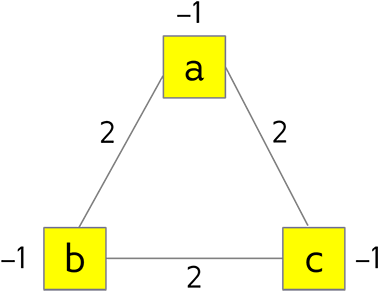
\includegraphics[width=0.4\columnwidth]{graphics/dwave_triangle_graph.png}
	\caption{A graph equivalent to QUBO describing three binary variables, where only one should be equal $1$ (true) \cite{d-wave_inc_d-wave_2022}.}
    \label{fig:dwave_triangle_graph}
\end{figure}

There of course are many cases that do not fit natural QUBO formulation discussed in \autoref{subsub:Natural_QUBO} nor are required penalties formulated as discussed in this section. For such cases a more general method is available. Please refer to \cite{glover_quantum_2019} for detailed explanation. It is also possible to use dedicated software libraries as discussed in \autoref{sub:qubo_tools}.
\subsection{Usefull Tools for formulating QUBOS}\label{sub:qubo_tools}
\section{Solving}
\subsection{Embedding}
\section{Performance}

\chapter{Problem}

\chapter{Conclusions and remarks}
\chapter{Scratchbook}
Ocean toolkit is the software suite currently used by DWave to solve computational problems. It consists of various submodules, each aimed at different stage of the process. The toolkit is freely available on Github \cite{DWGitHub}.

\bibliographystyle{plain}
\bibliography{ref} 

\end{document}